\documentclass[crop]{standalone}

\usepackage[dvipsnames]{xcolor}
\usepackage{tikz}

\usetikzlibrary{backgrounds}

\begin{document}
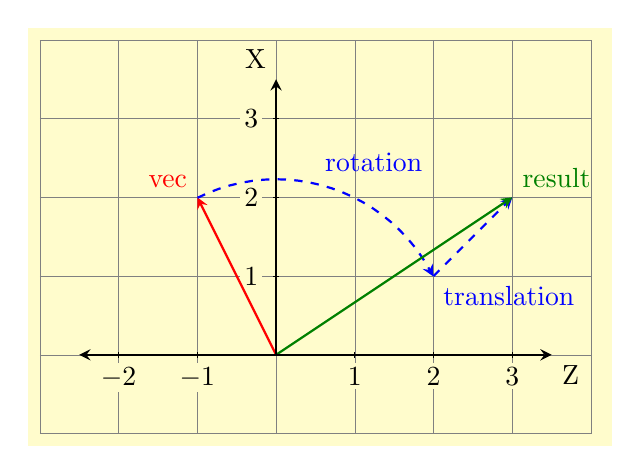
\begin{tikzpicture}[background rectangle/.style={fill=yellow!20}, show background rectangle]


	\draw[step=1cm,gray,very thin] (-3,-1) grid (4,4);

	\foreach \z in {-2,-1,1,2,3}
		\draw (\z cm,1pt) -- (\z cm,-1pt) node[anchor=north, inner sep=1.5pt, outer ysep=2pt, fill=yellow!20] {$\z$};
	\foreach \x in {1,2,3}
		\draw (1pt,\x cm) -- (-1pt,\x cm) node[anchor=east, inner sep=1.5pt, outer xsep=4pt, fill=yellow!20] {$\x$};


	\draw[thick,-stealth,red] (0,0) -- (-1,2) node[anchor=south east] {vec};
	\draw[blue,thick,domain=116.57:26.57,dashed,-stealth] plot ({2.23*cos(\x)}, {2.23*sin(\x)});
	\draw[thick,-stealth,dashed,blue] (2,1) -- (3,2);
	\node[blue,anchor=south west] at (0.5,2.2) {rotation};
	\node[blue,anchor=north west] at (2,1) {translation};
	\draw[thick,-stealth,Green] (0,0) -- (3,2) node[anchor=south west] {result};


	\draw[thick,stealth-stealth] (-2.5,0) -- (3.5,0) node[anchor=north west] {Z};
	\draw[thick,-stealth] (0,0) -- (0,3.5) node[anchor=south east] {X};


\end{tikzpicture}
\end{document}
